\chapter{Numbers 12}

\begin{figure}
  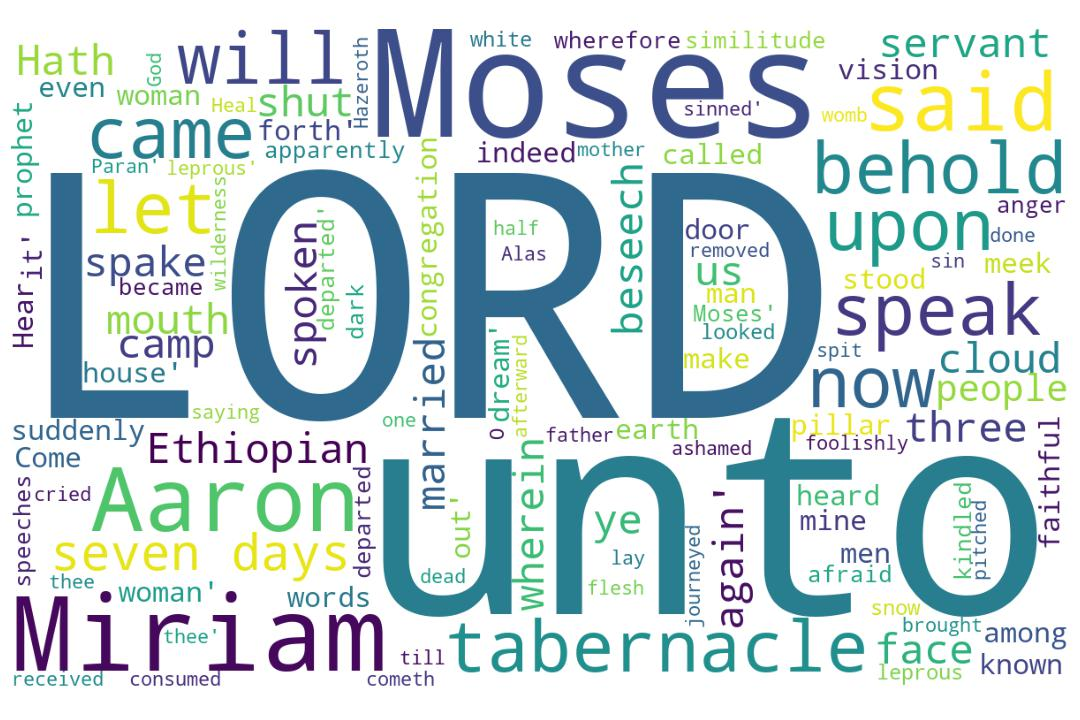
\includegraphics[width=\linewidth]{04OT-Numbers/Numbers12-WordCloud.jpg}
  \caption{Numbers 12 Word Cloud}
  \label{fig:Numbers 12 word Cloud}
\end{figure}

\marginpar{\scriptsize \centering \fcolorbox{bone}{lime}{\textbf{ABOUT THE LEADER}}\\ (Numbers 12:1-16) \begin{compactenum}[I.][8]
    \item \textbf{Authority Challenged} \index[scripture]{Numbers!Num 12:01}(Numbers 12:1)
    \item \textbf{Authenticity Confirmed} \index[scripture]{Numbers!Num 12:06--08}(Numbers 12:6-8)
    \item \textbf{Angered Kindled} \index[scripture]{Numbers!Num 12:10}(Numbers 12:10)
    \item \textbf{Arbitrated Clemency} \index[scripture]{Numbers!Num 12:14}(Numbers 12:14)
\end{compactenum}}


\footnote{\textcolor[cmyk]{0.99998,1,0,0}{\hyperlink{TOC}{Return to end of Table of Contents.}}}\footnote{\href{https://audiobible.com/bible/numbers_12.html}{\textcolor[cmyk]{0.99998,1,0,0}{Numbers 12 Audio}}}\textcolor[cmyk]{0.99998,1,0,0}{And Miriam and Aaron \fcolorbox{bone}{lime}{spake against} Moses because of the Ethiopian woman whom he had married: for he had married an Ethiopian woman.}
[2] \textcolor[cmyk]{0.99998,1,0,0}{And they said, Hath the LORD indeed spoken only by Moses? hath he not spoken also by us? And the LORD heard \emph{it}.}
[3] \textcolor[cmyk]{0.99998,1,0,0}{(Now the man Moses \emph{was} very meek, above all the men which \emph{were} upon the face of the earth.)}
[4] \textcolor[cmyk]{0.99998,1,0,0}{And the LORD spake suddenly unto Moses, and unto Aaron, and unto Miriam, Come out ye three unto the tabernacle of the congregation. And they three came out.}
[5] \textcolor[cmyk]{0.99998,1,0,0}{And the LORD came down in the pillar of the cloud, and stood \emph{in} the door of the tabernacle, and called Aaron and Miriam: and they both came forth.}
[6] \textcolor[cmyk]{0.99998,1,0,0}{And he said, \fcolorbox{bone}{lime}{Hear now} my words: If there be a prophet among you, \emph{I} the LORD will make myself known unto him in a vision, \emph{and} will speak unto him in a dream.}
[7] \textcolor[cmyk]{0.99998,1,0,0}{My servant Moses \emph{is} not so, who \emph{is} faithful in all mine house.}
[8] \textcolor[cmyk]{0.99998,1,0,0}{With him will I speak mouth to mouth, even apparently, and not in dark speeches; and the similitude of the LORD shall he behold: wherefore then were ye not afraid to speak against my servant Moses?}
[9] \textcolor[cmyk]{0.99998,1,0,0}{And the anger of the LORD was kindled against them; and he departed.}
[10] \textcolor[cmyk]{0.99998,1,0,0}{And the \fcolorbox{bone}{lime}{cloud departed} from off the tabernacle; and, behold, Miriam \emph{became} leprous, \emph{white} as snow: and Aaron looked upon Miriam, and, behold, \emph{she} \emph{was} leprous.}
[11] \textcolor[cmyk]{0.99998,1,0,0}{And Aaron said unto Moses, Alas, my lord, I beseech thee, lay not the sin upon us, wherein we have done foolishly, and wherein we have sinned.}
[12] \textcolor[cmyk]{0.99998,1,0,0}{Let her not be as one dead, of whom the flesh is half consumed when he cometh out of his mother's womb.}
[13] \textcolor[cmyk]{0.99998,1,0,0}{And Moses cried unto the LORD, saying, Heal her now, O God, I beseech thee.}\\
\\
\P \textcolor[cmyk]{0.99998,1,0,0}{And the LORD said unto Moses, If her father had but spit in her face, should she not be ashamed seven days? let her be shut out from the camp seven days, and \fcolorbox{bone}{lime}{after that} let her be received in \emph{again}.}
[15] \textcolor[cmyk]{0.99998,1,0,0}{And Miriam was shut out from the camp seven days: and the people journeyed not till Miriam was brought in \emph{again}.}
[16] \textcolor[cmyk]{0.99998,1,0,0}{And afterward the people removed from Hazeroth, and pitched in the wilderness of Paran.}